\chapter{Global Supercoiling in \emph{Aevol}}
\label{chap:aevol}

In this chapter, I present the first main line of work of that I undertook during my Ph. D., in which I implemented a model of the effect of DNA supercoiling on gene transcription into the \emph{Aevol} \emph{in silico} experimental evolution platform, in order to study the possible epistatic interactions between mutations that regulate the supercoiling level and other kinds of mutations.

\section{Introduction}
\label{sec:aevol_intro}

In the \emph{Long-Term Evolution Experiment}, started by Richard Lenski in 1988~\citep{lenski1991}, 12 populations of \emph{E. coli}, originating from the same ancestral strain, were placed to evolve in a new environment, a glucose-limited medium.
Every day since the beginning of the experiment, which is still running, a sample from each population has been propagated into fresh medium, resulting in the longest-running evolution experiment in the lab, and demonstrated that fitness can keep on increasing for much longer than originally expected in a constant environment~\citep{good2017}.
As sequencing capacity and synthetic biology developed in the late 1990s and early 2000s, identifying the precise DNA mutations underpinning these increases in fitness became possible.
Mutations in the \emph{fis} and \emph{topA} gene were thus found to lead to an increased growth rate in the conditions of the experiment, as well as to an increase in the basal supercoiling level of the cells bearing these mutations~\citep{crozat2005}.
\textbf{Devrait plutôt aller dans l'intro globale ?
Tel quel ça pose la question du rôle de la superhélicité dans l'évolution mais il n'y a pas (dans Crozat 2005 ou 2010) d'étude des suites évolutives de ces mutations de superhélicité.}

As mutations in genes regulating the level of supercoiling in \emph{E. coli}, such as \emph{topA} and \emph{fis}, were shown to increase fitness in the LTEE, we sought to investigate whether these mutations, by globally altering the regulatory landscape of the cell, could open up new evolutionary pathways and thereby speed up evolution, that is display positive epistasis with other mutations.
In order to explore this theoretical possibility without having to resort to wet-lab experiments, I resorted to the \emph{in silico} experimental evolution toolbox, using the \emph{Aevol} platform.


\section{The \emph{Aevol} model}
\label{sec:aevol_model}

\begin{figure}[H]
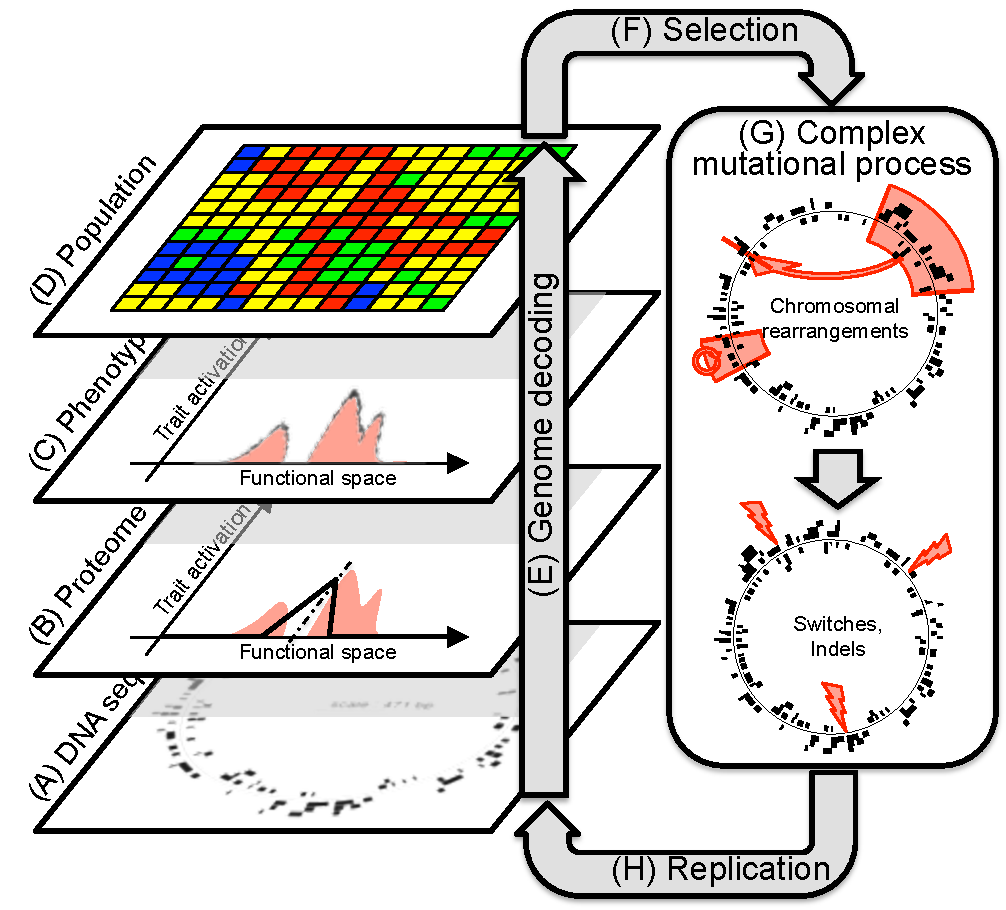
\includegraphics[width=\textwidth]{aevol/images/aevol.pdf}
\caption[Overview of the \emph{Aevol} model]{Broad overview of the \emph{Aevol} model.}
\label{fig:aevol_model}
\end{figure}

\subsection{Overview}

The \emph{Aevol} platform, developed in the Inria Beagle team~\citep{rutten2019}, is a software suite designed to run artificial evolution experiments on a computer, rather than at the bench.
As an excellent and very thorough description of \emph{Aevol} (in French) can be found in~\cite{liard2020b}, the following presentation of the model will be shorter and to the point.
Figure~\ref{fig:aevol_model} provides a comprehensive overview of the evolutionary algorithm at the core of \emph{Aevol}.
It follows the evolution over a given number of generations of a population of individuals that are defined by their genome, encoded as a circular string of nucleotides (A), in an environment described by an optimal phenotype.
At every generation, the genome of every individual is transcribed into RNA then translated into proteins (B), following the ``central dogma of molecular biology``~\citep{crick1958}.
These proteins are then mapped to an abstract phenotypic space (C), and the resulting phenotype is compared to the optimal phenotype in order to compute the fitness of the individual.
The population is laid out on a square grid (D), and the ancestor of the new individual in each cell is chosen at random among the neighboring individuals, proportionally to their fitness (F).
Once chosen, its genome undergoes a series of random mutations, including genomic rearrangements as well as local mutations (G), in order to obtain the genome of its successor in the next generation (H).

\subsection{The Genotype-Phenotype Map in \emph{Aevol}}

A genome in \emph{Aevol} consists in a sequence of binary characters ($0$ or $1$), representing a double-stranded circular sequence of DNA.
The genome sequence explicitly describes the first, or leading, strand, while the second, or lagging, strand is obtained by taking the complement of the sequence (replacing $0$ by $1$ and vice-versa).
The decoding algorithm starts by looking for sequences that code for viable RNAs, reading the leading strand left-to-right and the lagging strand right-to-left.
An RNA starts with a promoter sequence, which has to match a consensus sequence up to a few errors, and ends with a hairpin-like terminator.
Then, each RNA is scanned for ribosome binding sites followed by a 3-nucleotide start codon.
Reading continues until a stop codon is found in the same frame, and the resulting string of codons is then translated into a protein.

As the genetic alphabet is binary in \emph{Aevol}, there are 8 different 3-nucleotide codons, and therefore 6 codons left to encode protein data.
These codons are grouped into three pairs, each respectively encoding the width $w$, height $h$, and mean position $m$ of a kernel function from $[0, 1]$ to $[0, 1]$ representing the function of the protein in the abstract phenotypic space.
To obtain the expression $e$ of the protein, the height of the triangle is weighted by the difference $d$ of the promoter sequence to the consensus sequence: $e = 1 - \frac{d}{1+d_{max}}$, where $d_{max} = 4$.
Finally, in order to compute the complete phenotype of the individual from the set of its proteins, all the kernel functions are summed using Łukasiewicz operators, capping at $1$ the maximum value of the phenotype function.

\subsection{Fitness}

Once the phenotype of an individual has been decoded from its genome, we can compute its fitness.
As the environment is specified in \emph{Aevol} using an optimal phenotype, we first compute a gap value as the integral of the absolute value of the difference between the phenotype of the individual and the optimal phenotype, taken from $0$ to $1$ (the $L^1$ distance between the functions).
Then, we compute the fitness as the inverse exponential of the gap, multiplied by a selection coefficient: the higher this coefficient, the larger the difference in fitness between individuals with the same difference in gap.

\subsection{Mutational Operators}

Once the ancestor of a new individual has been chosen, a set of random mutations are applied to its genome to obtain the new genome.
These mutations are split in two classes, depending on the proportion of the genome that they can modify.
Genomic rearrangements, possibly affecting the whole genome, comprise large-scale deletions and duplications, inversions, and translocations.
Local mutations comprise small insertions and deletions (indels), and switches.

\subsection{Modeling DNA Supercoiling in \emph{Aevol}}

In order to model the effect of supercoiling on gene transcription in \emph{Aevol}, I chose to start with the simplest approximation, considering that the supercoiling level is constant along the genome and over time, which can be interpreted as considering the spatial and temporal average of a dynamic supercoiling level.
To implement this model inside \emph{Aevol}, I changed the genotype of individuals by adding, alongside the string-of-nucleotide genome, a single parameter $\gamma$, which represents the variation in the supercoiling level $\sigma$ of this individual compared to a reference supercoiling level $\sigma_0$: $\gamma = \frac{\sigma-\sigma_0}{\sigma_0}$.

\paragraph{Gene Expression}
To keep the model as simple as possible, supercoiling linearly effects the transcription level of all genes, adding a term into the computation of their expression level:

\begin{equation}
e = (1 - \frac{d}{1+d_{max}}) \cdot (1 - \gamma)
\label{eq:aevol_sc}
\end{equation}

When $\gamma$ is 0, the supercoiling level is equal to the baseline, resulting in no change to the expression level.

\paragraph{Mutational Operator}
In order to model mutations resulting in a new supercoiling level, I chose a continuous variation model: when an individual reproduces, we first use a Bernoulli trial with probability $p$ to decide whether its supercoiling level should change or remain constant during reproduction.
Then, if the supercoiling level changes, we choose a delta $\delta\gamma$ according to a normal distribution $\mathcal{N}(0, s^2)$, and finally set the supercoiling level $\gamma'$ of the offspring as $\gamma' = \gamma + \delta\gamma$.
The parameters of these laws are given as parameters to the \emph{Aevol} simulation, with the following values: $p = 10^{-1}$ and $s^2 = 10^{-2}$.


\section{Results}
\label{sec:aevol_results}

\begin{figure}[H]
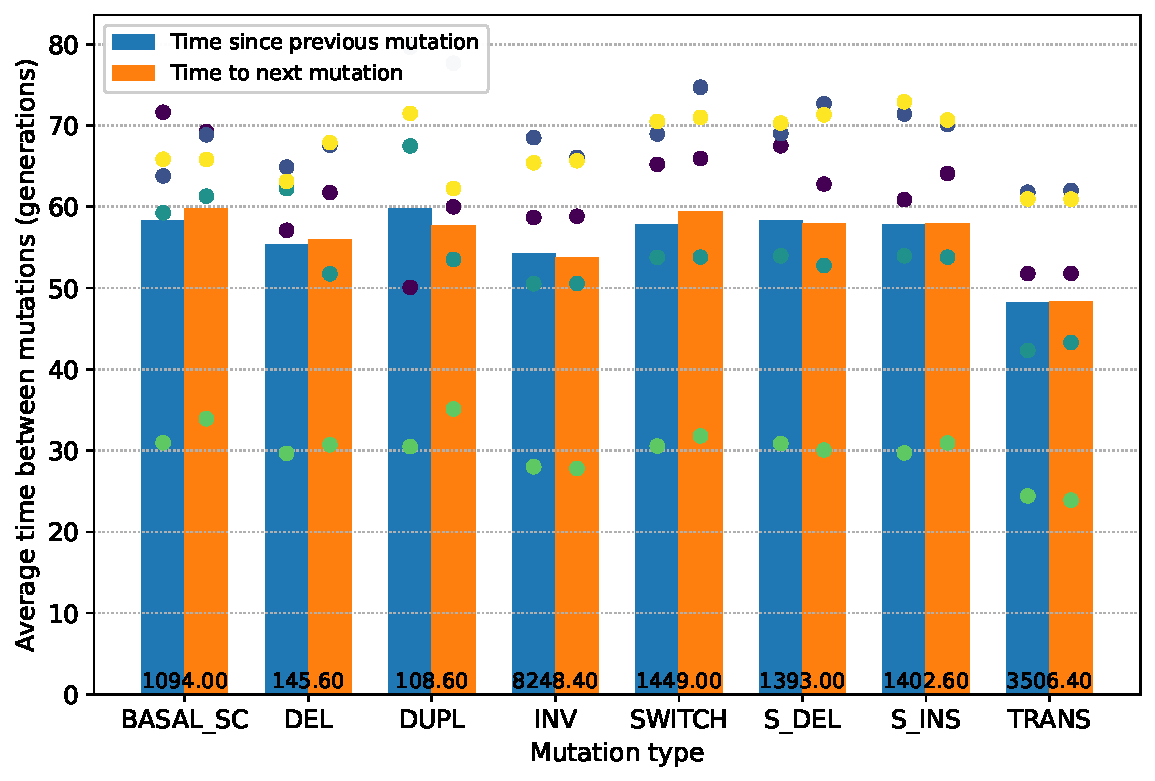
\includegraphics[width=\textwidth]{aevol/images/with_sc_mut_time_150k_995k.pdf}
\caption{I need to remember the mutation types}
\end{figure}

\subsection{Experimental Protocol}

Using this version of \emph{Aevol}, I compared the evolution of populations in which supercoiling is impacted by mutations, and populations in which supercoiling is kept constant.


\section{Conclusion}
\label{sec:aevol_ccl}